\section{Diseño Arquitectónico del Sistema}

El desarrollo se fundamenta en un diseño modular que desacopla la fase de preparación de datos (ingesta) de la fase de consulta (inferencia). Como se aprecia en la Figura (\ref{fig:architecture}), el diseño establece una separación clara de responsabilidades a través de un orquestador híbrido.

\begin{figure}[H]
    \centering
    
\includegraphics[width=0.9\textwidth]{Ilustraciones/Architecture-1.pdf}
    \caption{Arquitectura general del \gls{rag} híbrido desarrollado para DiSeCan.}
    \label{fig:architecture}
\end{figure}

El servidor backend expone una interfaz de comunicación mediante una API REST desarrollada en Flask, separando visualmente la aplicación \textit{frontend} desarrollada a medida, de la maquinaria interna de Inteligencia Artificial que soporta el procesamiento de lenguaje.

\subsection{Modelado de Datos y \textit{Chunking} Consciente del Contexto}

Uno de los principales retos al tratar transcripciones de documentos parlamentarios es la pérdida de la autoría y la secuencia de los discursos cuando se trocean los textos. Para solucionarlo, se desarrolló un \textit{pipeline} de ingestión de textos fundamentado en los metadatos lógicos (véase el bloque offline de la Figura \ref{fig:architecture}).

\begin{figure}[H]
    \centering
    
\includegraphics[width=0.7\textwidth]{Ilustraciones/EntityRelation-1.pdf}
    \caption{Modelo de datos mostrando el puente entre el entorno relacional de metadatos tradicionales y el ecosistema semántico.}
    \label{fig:erdiagram}
\end{figure}

En lugar de fragmentar los textos de forma arbitraria por límites automáticos de \textit{tokens}, el diseño propuesto concatena toda intervención ininterrumpida de un mismo orador para construir un solo fragmento lógico. El mundo puramente relacional (proveniente de tablas unificadas en la base de datos SQL) da a luz a una nueva entidad: los \textit{Chunks}. Esta estructura posibilita la relación bidireccional entre la representación matemática de los \textit{embeddings}\footnote{Vectores matemáticos de alta dimensionalidad o \textit{arrays} en coma flotante que capturan la representación semántica latente y abstracta de cada oración} y el contexto estricto y originario del interviniente, mitigando la fragmentación caótica de intervenciones largas.

\subsection{Recuperación Híbrida y Reordenamiento de Resultados}

Para maximizar la precisión de recuperación e intentar neutralizar las alucinaciones estadísticas de los modelos generativos, el motor de recuperación se sustenta en una arquitectura de búsqueda \textit{multistage} o de extracción en múltiples pasos:

\begin{figure}[H]
    \centering
    
\includegraphics[width=0.8\textwidth]{Ilustraciones/Sequence_Diagram.pdf}
    \caption{Diagrama de secuencia abordando el flujo asíncrono en la atención y enrutado de preguntas ciudadanas.}
    \label{fig:sequence}
\end{figure}

El proceso de enrutado técnico detallado en la Figura \ref{fig:sequence} se rige por cinco etapas de refinamiento:
\begin{enumerate}
    \item \textbf{Pre-filtrado determinista (SQL):} En primera instancia, se aplican los requerimientos introducidos en la configuración visual de la interfaz, induciendo filtros rígidos del ecosistema relacional para delimitar el espacio de exploración únicamente a documentos habilitados (ej. por legislatura y fechas).
    \item \textbf{Recuperación Vectorial Semántica:} Mediante el sistema persistente \gls{chromadb} \cite{chromadb2025}, se computan qué fragmentos parlamentarios muestran la mayor densidad y correlación semántica al cotejar la representación latente de la pregunta empleando codificadores multi-idioma (como el modelo \textit{multilingual-e5-base} \cite{wang2022text}).
    \item \textbf{Recuperación Léxica Exacta:} Paralelamente, como salvoconducto técnico ante la conocida deficiencia que tienen las bases vectoriales para detectar nombres exactos de leyes o individuos singulares, se elabora un índice invertido en memoria con el algoritmo estadístico \gls{bm25} \cite{robertson2009probabilistic}.
    \item \textbf{Fusión Recíproca de Clasificación (\gls{rrf}):} Al obtener dos flujos de documentos potencialmente relevantes con sistemas de métricas y escalas no comparables, se unifica el conocimiento extraído empleando un enfoque sin requerimientos de calibración, validado históricamente para sistemas \textit{Rank Learning} \cite{cormack2009reciprocal}.
    \item \textbf{\gls{crossencoder} Reranking:} Como última barrera analítica, debido a su alto coste computacional, los mejores extractos fusionados son evaluados de manera conjunta (documento y pregunta al unísono) por una red afinada mediante conocimiento transferido de sistemas de pregunta-respuesta masivos como \textit{mMARCO} \cite{bonifacio2021mmarco}. Esto proporciona el ordenamiento ultra-preciso  final para entregar un contexto nítido al motor \gls{vllm}.
\end{enumerate}

\subsection{Interfaz de Usuario e Interacción Gráfica}

La usabilidad ciudadana fue materializada en una Interfaz de Usuario dedicada; desarrollada empleando una \textit{Single Page Application} (SPA) que imita fluidamente los perfiles corporativos y estéticos de las plataformas \gls{iatext} oficiales. Cuenta además con un rediseño condicional a entornos oscuros.

\begin{figure}[H]
    \centering
    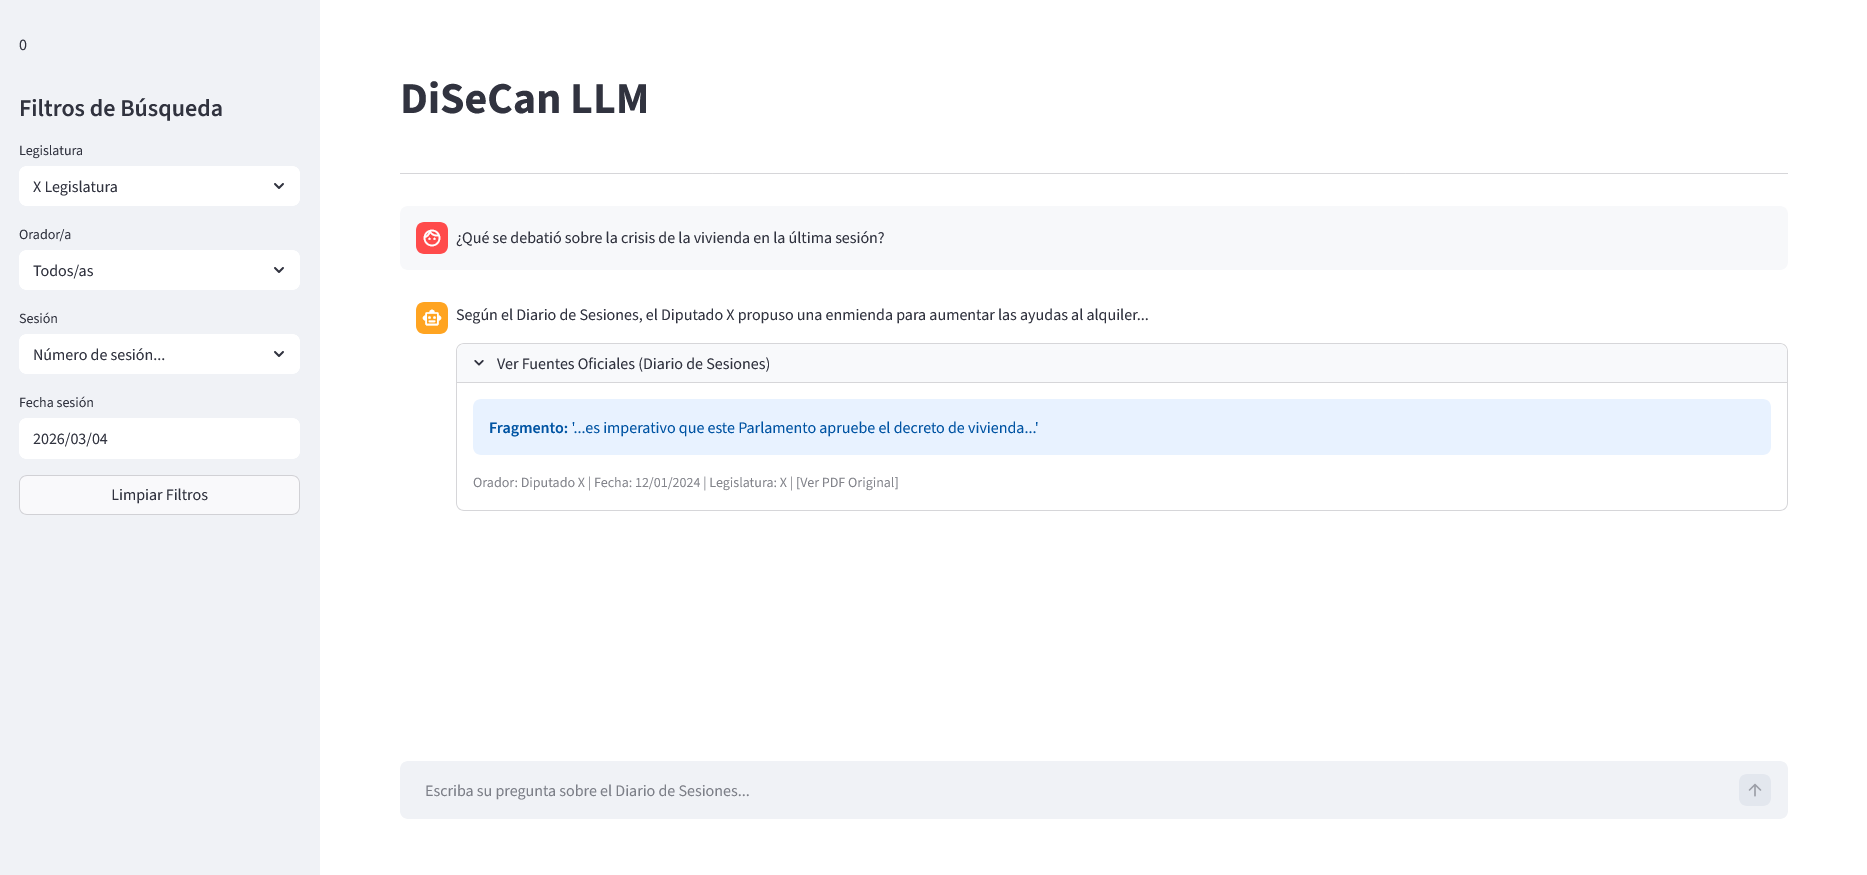
\includegraphics[width=0.8\textwidth]{Ilustraciones/mockuplight.png}
    \caption{Aspecto del sistema en Modo Claro (dispositivo tableta/escritorio).}
    \label{fig:mockuplight}
\end{figure}

\begin{figure}[H]
    \centering
    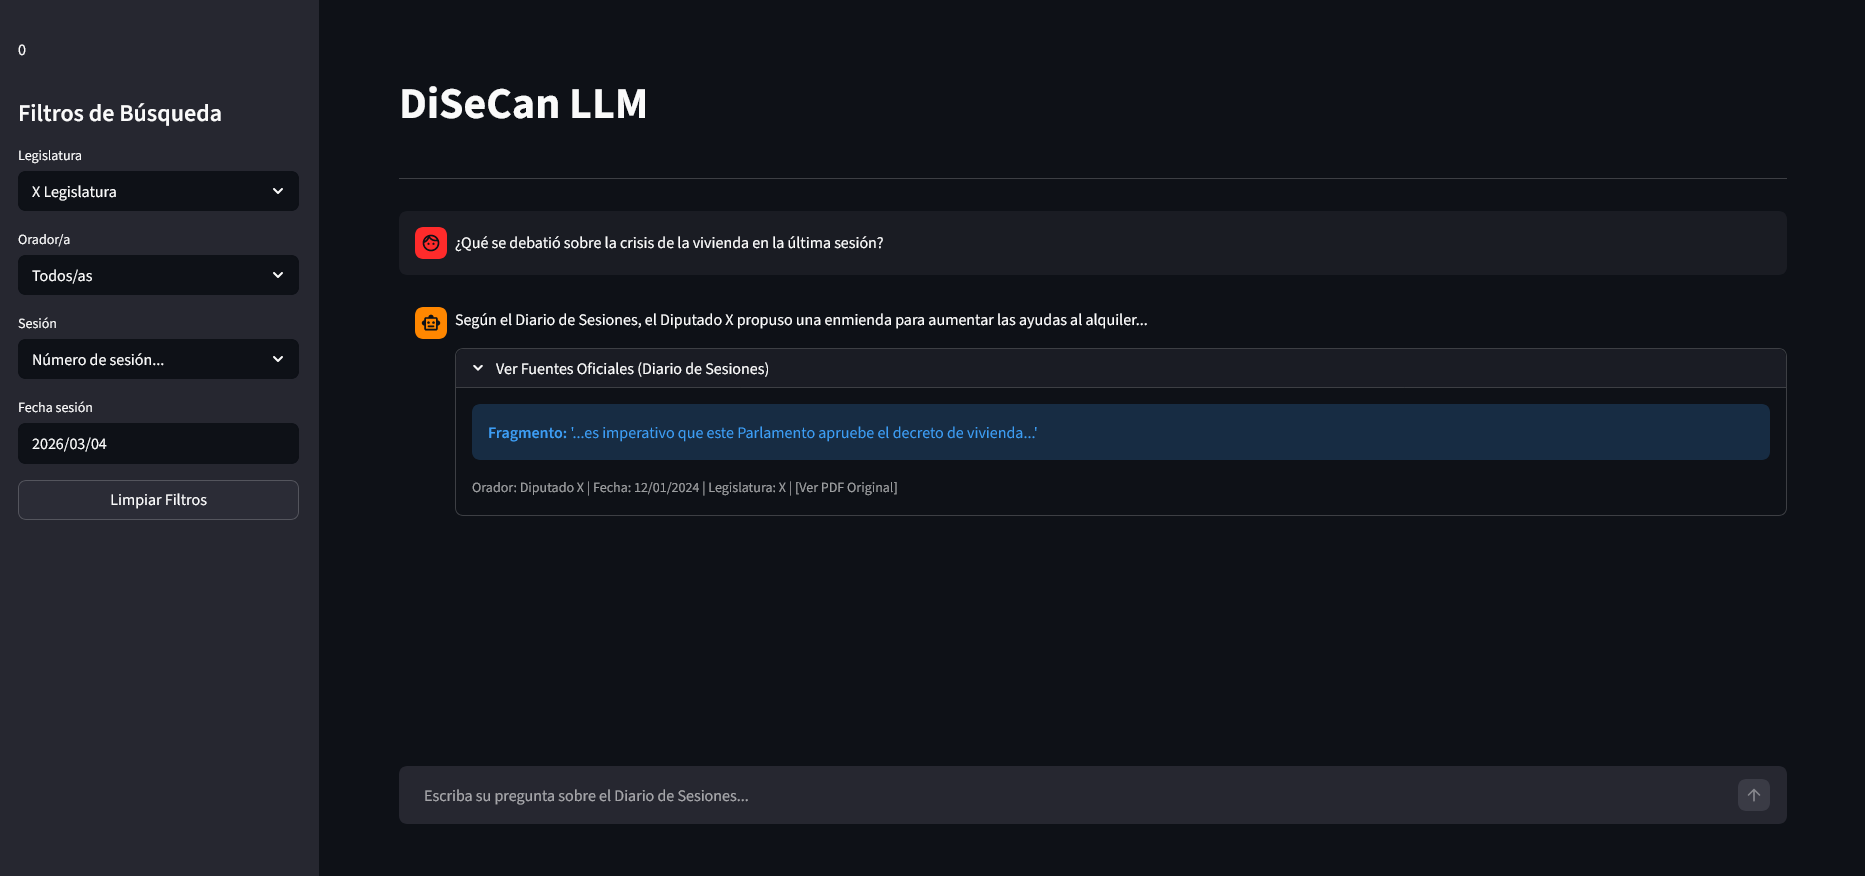
\includegraphics[width=0.8\textwidth]{Ilustraciones/mockupdark.png}
    \caption{Aspecto del sistema en el diseño invertido o Modo Oscuro.}
    \label{fig:mockupdark}
\end{figure}
